\documentclass[12pt,a4paper]{ctexart}
\usepackage{geometry,amsmath,amssymb,graphicx,booktabs,listings}
\geometry{left=2.7cm,right=2.7cm,top=2.5cm,bottom=2.5cm}
\setlength{\parindent}{2em}
\setlength{\parskip}{0.35em}
\lstset{language=C,basicstyle=\ttfamily\footnotesize,columns=fullflexible,keepspaces=true,breaklines=true,showstringspaces=false,aboveskip=0.6em,belowskip=0.8em}
\title{Datalab实验报告}
\author{朱家琛\quad 2025201895}
\date{}
\begin{document}
\maketitle

\section*{实验结果}

\begin{center}
\begin{tabular}{lclc}
\toprule
函数 & 得分 & 函数 & 得分 \\
\midrule
bitAnd & 1/1 & reverse & 3/3 \\
bitXor & 1/1 & logicalShift & 3/3 \\
samesign & 2/2 & leftBitCount & 4/4 \\
logtwo & 4/4 & float\_i2f & 4/4 \\
byteSwap & 4/4 & floatScale2 & 4/4 \\
float64\_f2i & 3/3 & floatPower2 & 4/4 \\
\bottomrule
\end{tabular}
\end{center}

\noindent\textbf{测试截图}

\begin{center}
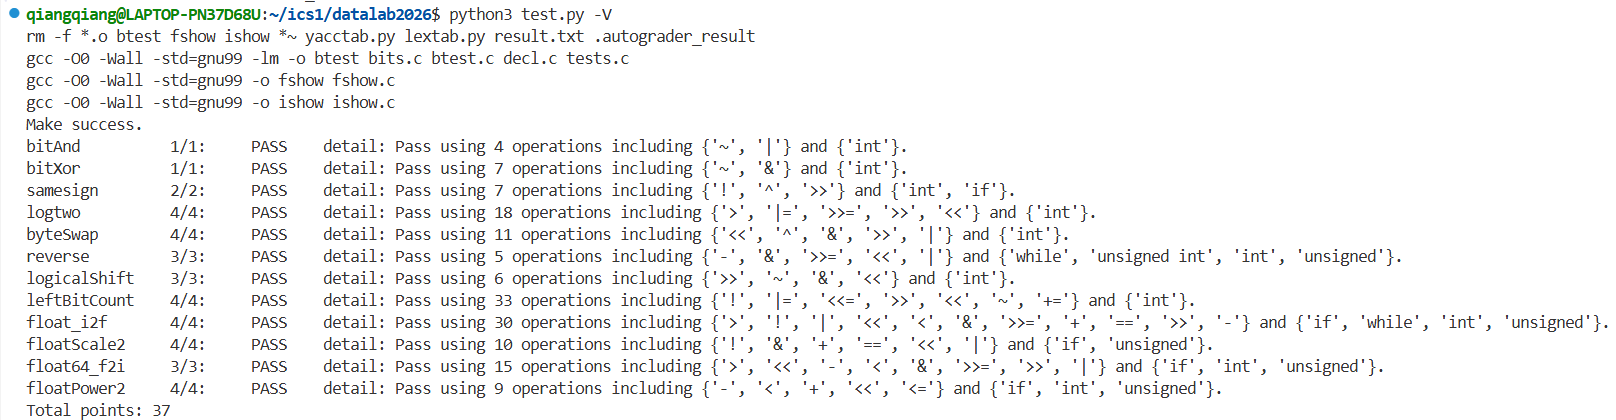
\includegraphics[width=\textwidth]{imgs/img1.png}
\end{center}

\section*{解题报告}

\noindent\textbf{亮点：} \texttt{logtwo} 和 \texttt{leftBitCount} 都采用分块二分的思路，分别确定最高位 1 的位置和前导 1 的个数；\texttt{byteSwap} 用异或差值直接交换字节；\texttt{float\_i2f} 处理了向偶数舍入及尾数进位。

\clearpage

\section{bitAnd}
题目只允许使用取反和按位或。根据德摩根律，\texttt{x \& y} 可以写成 \texttt{\char`\~(\char`\~x | \char`\~y)}。

具体看某一位：如果 $x$ 和 $y$ 都是 1，分别取反后都是 0，按位或仍是 0，最后取反得到 1。只要其中有一个是 0，取反后至少有一个是 1，按位或得到 1，最后取反得到 0。因此每一位的结果都与按位与相同。

\begin{lstlisting}
int bitAnd(int x, int y) {
    return  ~((~x)|(~y));
}
\end{lstlisting}

\section{bitXor}
异或在两位不同的时候为 1。处理时分别排除“两位都是 1”和“两位都是 0”：\texttt{\char`\~(x \& y)} 排除前一种情况，\texttt{\char`\~(\char`\~x \& \char`\~y)} 排除后一种情况。把两个结果按位与，留下的就只有 01 和 10 两种组合。

因此使用表达式
\[
\sim(x\mathbin{\&}y)\mathbin{\&}\sim(\sim x\mathbin{\&}\sim y).
\]
这里的每一步都只用到了题目允许的 \texttt{\char`\~} 和 \texttt{\&}。

\begin{lstlisting}
int bitXor(int x, int y) {
    return ~(x&y)&~(~x&~y);
}
\end{lstlisting}

\section{samesign}
非零整数的符号由最高位决定。将 $x$ 和 $y$ 分别算术右移 31 位，正数得到 0，负数得到全 1。两者异或后，如果结果为 0，就表示它们同为正数或同为负数，再用逻辑非将判断结果变成 1 或 0。

不过 0 的最高位也为 0，直接比较会把 0 和正数误判为同号。因此先检查零：当 $x=0$ 时，只有 $y=0$ 才返回 1；当 $x\ne0$ 且 $y=0$ 时返回 0。两个数都非零时再比较右移后的结果。

\begin{lstlisting}
int samesign(int x, int y) {
    if(!x)return !y;
    if(!y)return 0;
    return !((x>>31)^(y>>31));
}
\end{lstlisting}

\section{logtwo}
对于正整数 $v$，答案是其最高位 1 的编号。为了避免循环，按 16、8、4、2、1 位的顺序逐步缩小范围。

先比较 $v$ 与 \texttt{0xFFFF}。若 $v$ 更大，最高位至少在第 16 位，于是把 $v$ 右移 16 位，并在答案中记下 16；否则这一步移动 0 位。随后比较当前 $v$ 与 \texttt{0xFF}、\texttt{0xF}、\texttt{0x3}，分别决定是否再右移 8、4、2 位。经过这些步骤，当前 $v$ 只剩 1 或 2；\texttt{v >> 1} 就给出最后的 0 或 1。

比较表达式本身得到 0 或 1，把它左移相应位数就能产生 0 或 16、0 或 8 等移动量。得到的 16、8、4、2、1 各占答案中的一个独立二进制位，因此用按位或合并即可。

\begin{lstlisting}
int logtwo(int v) {
    int ans=0,shift=0;
    shift=(v>0xffff)<<4;
    ans|=shift;
    v>>=shift;
    shift=(v>0xff)<<3;
    ans|=shift;
    v>>=shift;
    shift=(v>0xf)<<2;
    ans|=shift;
    v>>=shift;
    shift=(v>0x3)<<1;
    ans|=shift;
    v>>=shift;
    ans|=v>>1;
    return ans;
}
\end{lstlisting}

\section{byteSwap}
先将字节编号换成位移量：第 $n$ 个字节对应 $n\ll3$ 位，第 $m$ 个字节对应 $m\ll3$ 位。分别把 $x$ 右移相应位数，再与 \texttt{0xFF} 按位与，就取得了两个字节，记为 $a$ 和 $b$。

令 $t=a\oplus b$。如果把 $t$ 与原来的 $a$ 异或，会得到 $b$；与原来的 $b$ 异或，则会得到 $a$。所以把 $t$ 左移到这两个字节的位置后合并，再与原数异或，就完成了交换，其余位不受影响。若两个编号相同，$t=0$，原数自然保持不变。

\begin{lstlisting}
int byteSwap(int x, int n, int m) {
    int sn=n<<3,sm=m<<3;
    int bn=(x>>sn)&0xff;
    int bm=(x>>sm)&0xff;
    int tmp=bn^bm;
    return x^((tmp<<sn)|(tmp<<sm));
}
\end{lstlisting}

\section{reverse}
从原数的最低位开始取位，再按相反方向逐个放进结果。每一轮用 \texttt{v \& 1} 取出当前最低位，将结果左移一位后把这一位接到末尾，接着将 $v$ 右移一位。这样，原数最先取出的最低位会逐步被推到结果的最高位。

必须固定做满 32 轮。如果在 $v$ 变成 0 时停止，尚未处理的前导零无法进入结果，最低位的 1 也可能到不了最高位。$v$ 和结果都使用无符号类型，右移时左侧补 0。

\begin{lstlisting}
unsigned reverse(unsigned v) {
    unsigned  int ans=0;
    int cnt=32;
    while(cnt--){
        ans=(ans<<1)|(v&1);
        v>>=1;
    }
    return ans;
}
\end{lstlisting}

\section{logicalShift}
对有符号负数执行 \texttt{x >> n} 时，左侧会补 1；逻辑右移要求左侧补 0。因此先进行普通右移，再构造一个掩码清掉补出的高位 1。

从 \texttt{1 << 31} 开始，将其算术右移 $n$ 位，会得到最高 $n+1$ 位为 1 的数；再左移一位，得到最高 $n$ 位为 1 的数；最后取反，得到最高 $n$ 位为 0、其余位为 1 的掩码。把 \texttt{x >> n} 与该掩码按位与，即为所需结果。$n=0$ 时掩码为全 1，$n=31$ 时只保留最低位。

\begin{lstlisting}
int logicalShift(int x, int n) {
    return (x>>n)&~(((1<<31)>>n)<<1);
}
\end{lstlisting}

\section{leftBitCount}
要数的是从最左边开始、在第一个 0 出现前连续有多少个 1。不能用循环逐位查找，就依次检查最高的 16、8、4、2、1 位。

检查最高 16 位时，将 $x$ 算术右移 16 位。如果这 16 位全是 1，右移结果会是全 1；取反后为 0，再做逻辑非便得到 1。把这个判断结果左移 4 位，可得到 0 或 16。如果得到 16，就把它记入答案，同时将 $x$ 左移 16 位，使尚未检查的部分来到最高位。后面的 8、4、2、1 位使用同样的方法处理。

这些移动量分别是 16、8、4、2、1，二进制位互不重叠，可用按位或累计。最后还要检查一次当前最高位，以处理连续 32 位都为 1 的情况。

\begin{lstlisting}
int leftBitCount(int x) {
    int ans=0,shift=0;
    shift=(!~(x>>16))<<4;
    ans|=shift;
    x<<=shift;
    shift=(!~(x>>24))<<3;
    ans|=shift;
    x<<=shift;
    shift=(!~(x>>28))<<2;
    ans|=shift;
    x<<=shift;
    shift=(!~(x>>30))<<1;
    ans|=shift;
    x<<=shift;
    shift=(!~(x>>31));
    ans|=shift;
    x<<=shift;
    shift=(!~(x>>31));
    ans+=shift;
    return ans;
}
\end{lstlisting}

\section{float\_i2f}
单精度浮点数有 1 位符号、8 位指数和 23 位尾数。规格化数还隐含一个最高位 1，因此实际可保存 24 位有效数字。转换时，先单独处理 $x=0$；再取出符号位，用无符号变量保存 $x$ 的绝对值。对负数先把它放进无符号变量，再对该变量取负，可以处理绝对值为 $2^{31}$ 的最小负数。

不断右移绝对值，数出最高位 1 位于第 $p$ 位。此时绝对值可写成 $1.xxx\times2^p$，指数域为 $p+127$。如果 $p<24$，所有有效位都装得下：将整数左移到最高位 1 对准隐藏位，再填入符号、指数和尾数，不需要舍入。

如果 $p\geq24$，需要右移 $p-23$ 位，只保留最高 24 位。被移走的低位决定是否进位：小于被舍弃部分的一半就不进位，大于一半就进位；恰好等于一半时，检查保留部分的最低位，若为 1 就进位，使最终保留部分为偶数。如果保留部分全是 1，进位可能跨过尾数进入指数域，组合位表示时也要让这一进位正确发生。

\begin{lstlisting}
unsigned float_i2f(int x) {
    if(!x)return 0;
    unsigned sign=x&0x80000000;
    unsigned x1=x,result;
    if(x<0)x1=-x1;
    unsigned tmp=x1;
    int p=0;
    while(tmp>>1){
        tmp>>=1;
        p++;
    }
    if(p<24){
        return sign|(((p+126)<<23)+(x1<<(23-p)));
    }
    int shift=p-23;
    unsigned retained=x1>>shift;
    result=sign|(((p+126)<<23)+retained);
    unsigned discarded=x1&((1<<shift)-1);
    unsigned half=1<<(shift-1);
    if(discarded>half)result++;
    else if(discarded==half)if(retained&1)result++;
    return result;
}
\end{lstlisting}

\section{floatScale2}
先取出符号和指数，按浮点数类别处理。指数全为 1 时，数值是无穷或 NaN：无穷乘 2 不变，NaN 按题目要求原样返回，因此直接返回原参数。

指数为 0 时，输入是零或非规格化数。它没有隐藏的最高位 1，乘 2 可以直接将尾数左移一位，并保留符号位。最高的尾数位若因此进入指数域，结果会自然变成规格化数。其余情况是规格化数，乘 2 只需让指数加 1。唯独原指数为 254 时需要单独处理：再加 1 会得到全 1 指数，此时要把尾数清零，返回相应符号的无穷，否则会错误地得到 NaN。

\begin{lstlisting}
unsigned floatScale2(unsigned uf) {
    unsigned sign=uf&0x80000000;
    unsigned exp=uf&0x7f800000;
    if(exp==0x7f800000)return uf;
    if(!exp)return sign|((uf&0x7fffffff)<<1);
    if(exp==0x7f000000)return sign|0x7f800000;
    return uf+0x00800000;
}
\end{lstlisting}

\section{float64\_f2i}
双精度浮点数的高 32 位包含符号位、11 位指数和尾数的高 20 位，低 32 位包含剩余尾数。先从高 32 位取出符号和指数。指数域的偏置是 1023，因此真实指数为 $E=exp-1023$。

若 $exp<1023$，数的绝对值小于 1，向零取整后为 0；若 $exp>1054$，真实指数超过 31，结果超出 32 位有符号整数范围，返回规定的溢出值。无穷和 NaN 的指数同样落在后一类。

对中间范围的数，把规格化数隐藏的最高位 1 放在一个 32 位无符号数的第 31 位，再接上尾数的最高 31 位：其中 20 位来自高半部分，其余 11 位来自低半部分。此时构造出的数相当于把有效数字乘了 $2^{31}$，而原数要乘 $2^E$，所以还需右移 $31-E=1054-exp$ 位。右移丢掉低位，正好实现向零取整。最后按照符号加上正负，并分别检查范围：正数不能超过 \texttt{0x7FFFFFFF}，负数的绝对值不能超过 \texttt{0x80000000}。

\begin{lstlisting}
int float64_f2i(unsigned uf1, unsigned uf2) {
    unsigned sign=uf2>>31;
    unsigned exp=(uf2>>20)&(0x7ff);
    if(exp<1023)return 0;
    if(exp>1054)return 0x80000000;
    unsigned val=0x80000000|((uf2&0xfffff)<<11)|(uf1>>21);
    val>>=(1054-exp);
    if(sign){
        if(val>0x80000000)return 0x80000000;
        return -val;
    }
    else{
        if(val>0x7fffffff)return 0x80000000;
        return val;
    }
    return val;
}
\end{lstlisting}

\section{floatPower2}
$2^x$ 始终为正，符号位固定为 0。在规格化范围 $-126\leq x\leq127$ 内，它的有效数字是 $1.0$，尾数域全为 0，只要把 $x+127$ 放入指数域即可。

当 $-149\leq x<-126$ 时，结果是非规格化数。非规格化数的最低一位表示 $2^{-149}$，所以 $2^x$ 对应把尾数域的第 $x+149$ 位设为 1。若 $x<-149$，数值比最小非零编码还小，返回 0；若 $x>127$，超出有限数范围，返回正无穷 \texttt{0x7F800000}。

\begin{lstlisting}
unsigned floatPower2(int x) {
    if(x<-149)return 0;
    if(x<-126)return 1<<(x+149);
    if(x<=127)return (x+127)<<23;
    return 0x7f800000;
}
\end{lstlisting}

\section*{常用思路总结}

整数题主要利用位运算恒等式、移位和掩码处理指定的位；不方便使用分支或循环时，可以把比较结果转成 0 或位移量，分块处理。浮点题先拆出符号、指数和尾数，再按不同编码范围分别处理；丢弃有效位时还要考虑舍入和溢出。

\end{document}
